\documentclass{beamer}
\beamertemplatenavigationsymbolsempty
\usepackage{graphicx}
\usepackage{listings}
\lstset{
    breaklines=true,
    numbers=left,
    numberstyle=\scriptsize,
    frame=leftline,
    basicstyle=\ttfamily}

% TODO
%  * use \begin{frame}[fragile] with code examples


\begin{document}
\begin{frame}

    {\LARGE Merged Mining, SatoshiLabs, GeneralBytes}\\
    \vspace{7mm}
    {\Large Ondrej Sika \lstinline|<ondrej@ondrejsika.com>|}\\
    \vspace{7mm}
    {\large Slush Pool (\url{mining.bitcoin.cz})}\\
    \vspace{7mm}
    19. 8. 2015, Bitcoin Meetups Bern, Switzerland\\

\end{frame}

\begin{frame}

    {\LARGE Ondrej Sika}\\

    \vspace{5mm}

    - Work on mining pool (backend)\\
    - Bitcoin, Namecoin, Python/Twisted\\

    \vspace{10mm}

    {\LARGE Slush pool}\\

    \vspace{5mm}

    - First mining pool, founded 2011\\
    - Creator of stratum mining protocol\\
    - 20 000 miners, 5\% network hashrate\\

\end{frame}

\begin{frame}

    {\LARGE Mining, why?}\\

    \vspace{5mm}

    - trustless timestamping\\
    - distribution of coins\\

\end{frame}

\begin{frame}

    {\LARGE Namecoin}\\

    \vspace{5mm}

    - fork of Bitcoin\\
    - first altcoin\\
    - additional value - decentralized DNS\\

    \vspace{7mm}

    {\LARGE Why Namecoin?}\\

    \vspace{5mm}

    - same algorythm as bitcoin\\
    - most profitable mining\\

\end{frame}

\begin{frame}

    {\LARGE Blockchain}\\

    \vspace{5mm}

    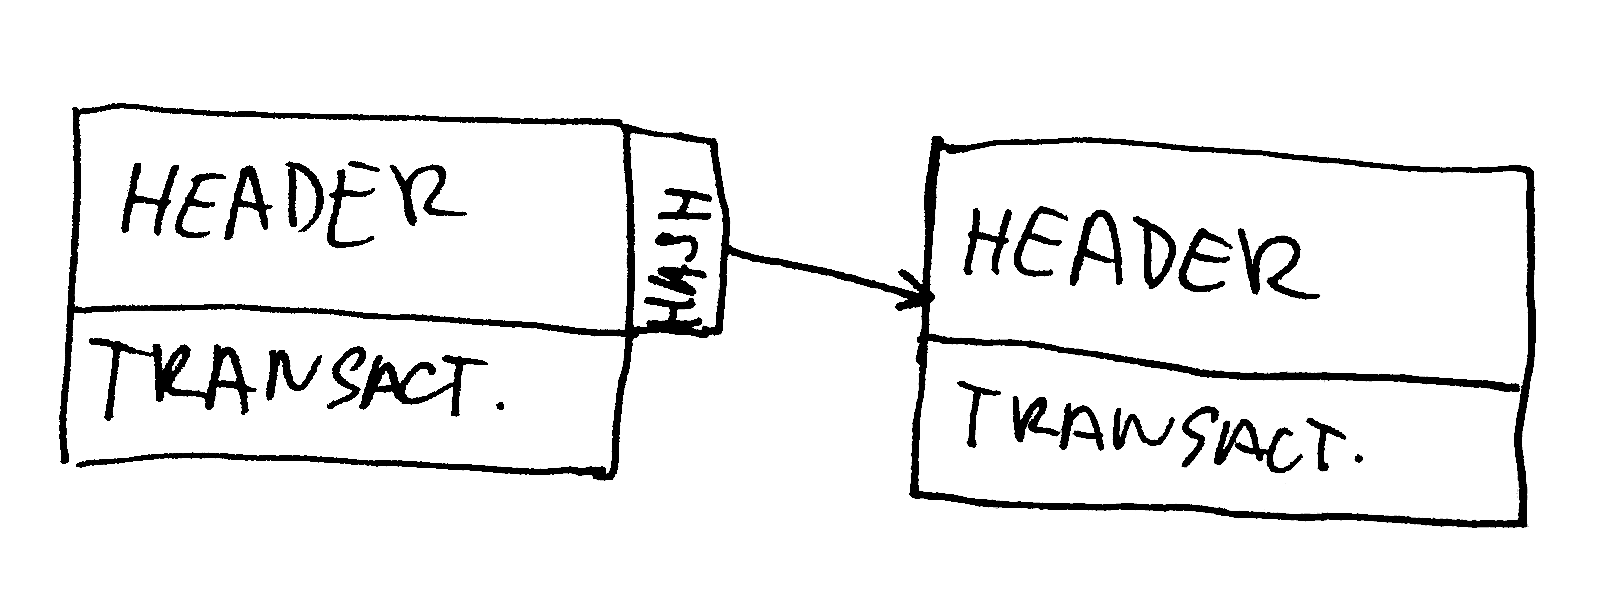
\includegraphics[scale=0.185]{img/blockchain}

\end{frame}

\begin{frame}

    {\LARGE Block}\\

    \vspace{5mm}

    - keep transaction information\\
    - some additional data\\

    \vspace{5mm}

    - header\\
    - transactions\\

\end{frame}

\begin{frame}

    {\LARGE Block Header}\\

    \vspace{5mm}

    - version\\
    - hashPrevBlock\\
    - hashMerkelRoot\\
    - time\\
    - bits (difficulty)\\
    - nonce\\

\end{frame}

\begin{frame}[fragile]

    {\LARGE Proof of Work}\\

    \vspace{5mm}

    "A proof of work is a piece of data which was difficult (costly, time-consuming) to produce so as to satisfy certain requirements"\\

    \vspace{5mm}

    \begin{verbatim}
"Hello, world!0" => 1312af178c253f84...
"Hello, world!1" => e9afc424b79e4f6a...
"Hello, world!2" => ae37343a357a8297...
.
.
"Hello, world!4248" => 6e110d98b388e...
"Hello, world!4249" => c004190b822f1...
"Hello, world!4250" => 0000c3af42fc3...
    \end{verbatim}

\end{frame}

\begin{frame}

    {\LARGE Merged Mining, why?}\\

    \vspace{5mm}

    - mining multiple coins with one hashrate\\
    - better security of altcoin\\

\end{frame}

\begin{frame}

    {\LARGE Auxiliary POW}\\

    \vspace{5mm}

    "This is the way that merged mining can exist; it is the relationship between two blockchains for one to trust the other's work as their own and accept AuxPOW blocks."\\

\end{frame}

\begin{frame}

    {\LARGE Bitcoin Coinbase}\\

    \vspace{5mm}

    - Input of first transaction in block\\
    - 100 Bytes for free use\\

    \vspace{5mm}

    - block height\\
    - flags\\
    - merged mining prefix\\
    - namecoin prevhash\\
    - ...\\

\end{frame}

\begin{frame}

    {\LARGE Principle of Aux POW}\\

    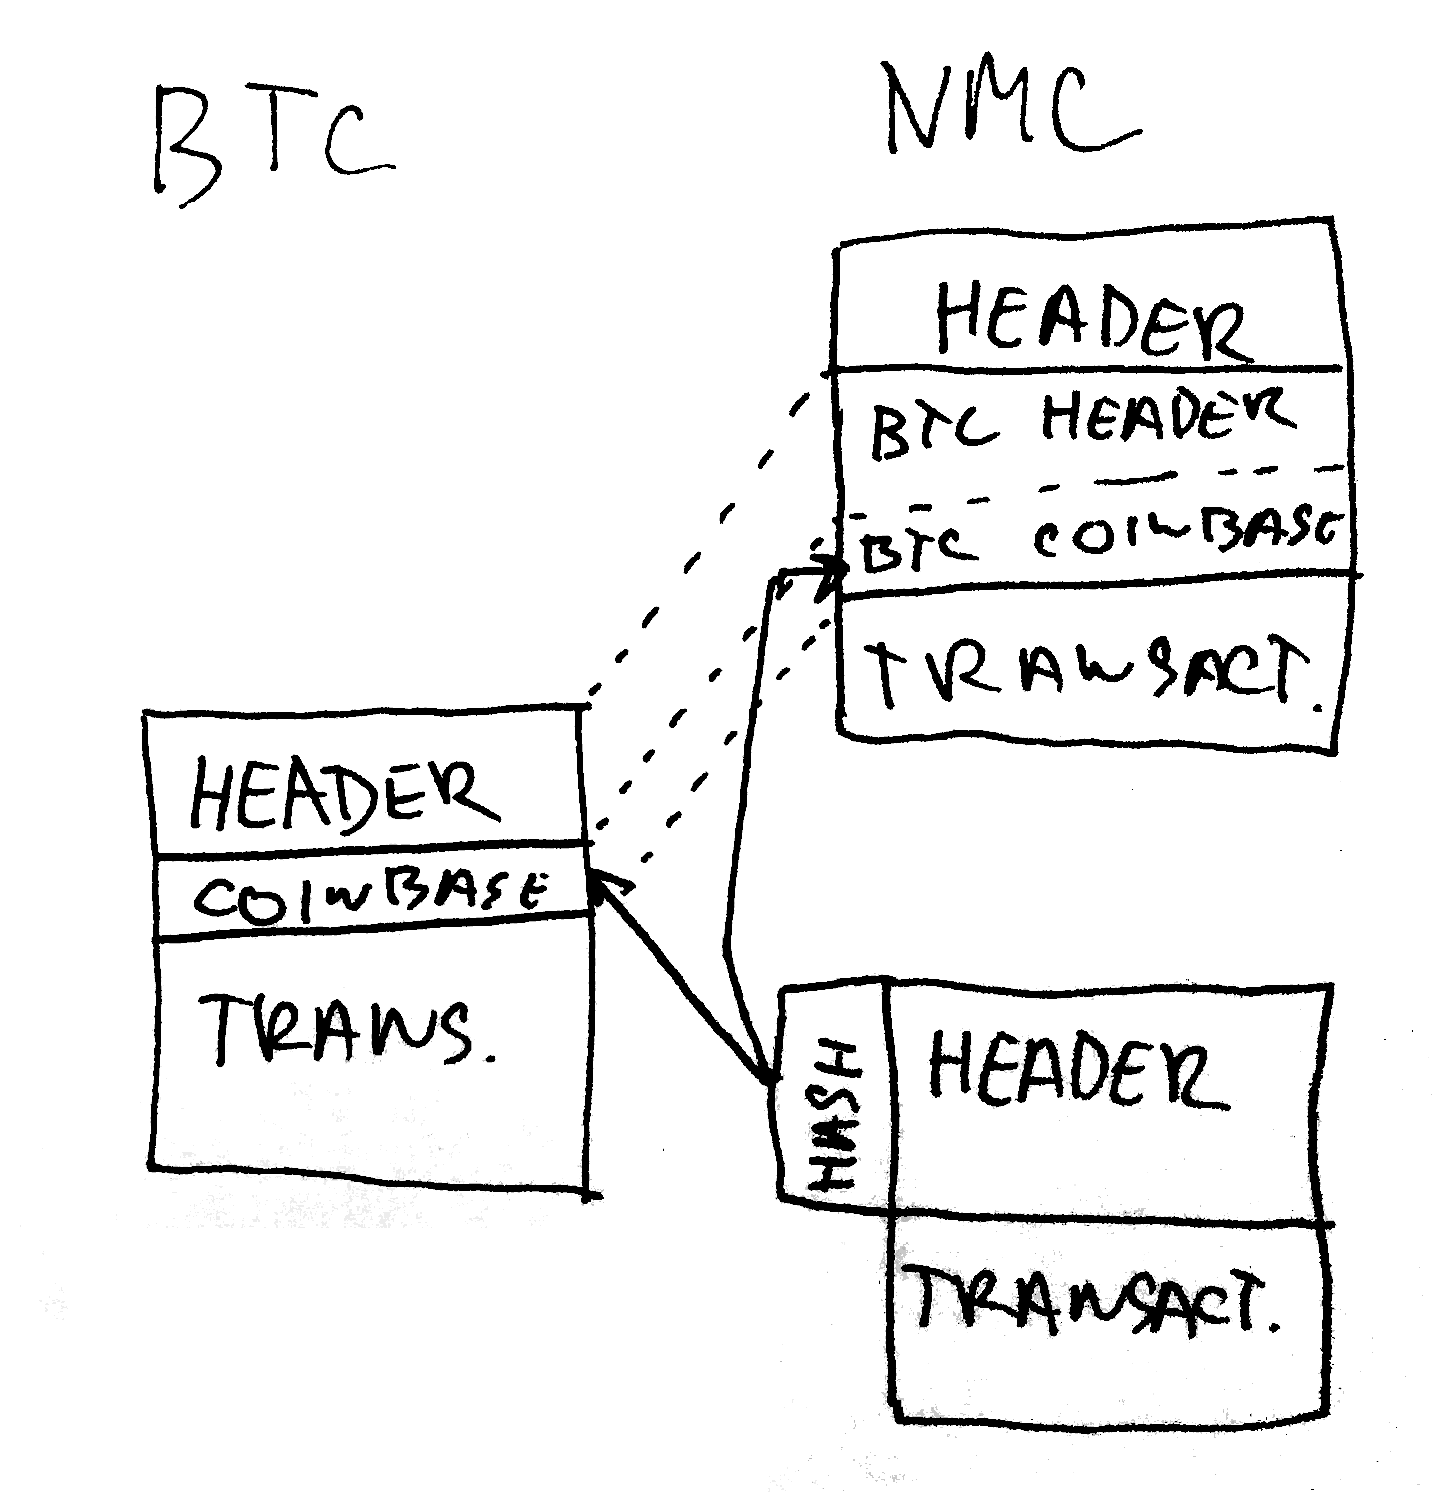
\includegraphics[scale=0.15]{img/principle_of_auxpow}

\end{frame}

\begin{frame}

    {\LARGE SatoshiLabs}\\

    \vspace{5mm}

    - Trezor\\
    - MyTrezor\\
    - Slush Pool\\
    - CoinMap 2.0\\

\end{frame}

\begin{frame}

    {\LARGE Trezor}\\

    \vspace{5mm}

    - first hardware wallet\\
    - utimate safe\\
    - hierarchic deterministic wallet (bip32, bip44)\\
    - multiple coins\\

    !!! IMG OF TREZOR !!!  % FIXME

\end{frame}

\begin{frame}

    {\LARGE MyTrezor}\\

    \vspace{5mm}

    - web client for Trezor\\
    - multiple accounts\\
    - for Bitcoin and Bitcoin Testnet only\\

    !!! SCREEN OF MYTREZOR !!!  % FIXME

\end{frame}

\begin{frame}

    {\LARGE Other trezor wallets}\\

    \vspace{5mm}

    - electrum, electrum ltc\\

    \vspace{10mm}

    {\LARGE Mobile wallets}\\

    \vspace{5mm}

    - mycelium\\

\end{frame}

\begin{frame}

    {\LARGE Coinmap 2.0}\\

    \vspace{5mm}

    - \url{http://coinmap.org}

    !!! SCREEN OF COINMAP !!!  % FIXME

\end{frame}

\begin{frame}

    {\LARGE GeneralBytes - Bitcoin ATMs}\\

    \vspace{5mm}

    !!! IMG !!!  % FIXME


\end{frame}

\begin{frame}

    {\LARGE GeneralBytes - Facts}\\

    \vspace{5mm}

    \begin{tabular}{lp{8cm}}
    - 9/2013 & Company founded in Prague Czech Republic\\
    - 2/2014 & First one-way machine put into production (BATM1)\\
    - 5/2014 & First Bitcoin ATM in world to feature fingerprint reader (BATM2)\\
    - 7/2014 & First Bitcoin ATM in world to allow you to implement support for your own coin and sell it on ATM (see github howto)\\
    - 8/2014 & First Bitcoin ATM in world to have Bitcoin Point-Of-Sale functionality on the ATM\\
    \end{tabular}

\end{frame}

\begin{frame}

    \begin{tabular}{lp{8cm}}
    - 11/2014 & Ported its ATM software to run on Robocoin machines. (15 robocoins are running GB software as of now including World’s first Bitcoin ATM in Vancouver)\\
    - 3/2015 & New Two-way(BATM3) model bitcoin ATM presented in London.\\
    - 6/2015 & First BATM3 machines deployed by customers world-wide.\\
    - 8/2015 & 82\% of 2-way machines in United Kingdom are running GB software. 100\% of bitcoin atms in Czech Republic running GB software. 85 in total machines sold worldwide.\\
    \end{tabular}

\end{frame}

\begin{frame}

    {\LARGE What next?}\\

    \vspace{5mm}

    - More GB ATM deployments around the world.\\
    - Our software ported to competing ATMs. No comment on which.\\
    - New features introduced on the ATM (like remittance)\\
    - New non-ATM products to be introduced...\\

\end{frame}

\begin{frame}

    {\LARGE Here is one of them: Bitcoin-only stand alone POS}\\

    \vspace{5mm}

    - About to leave incubation phase (in real life testing since 3/2015)\\
    - Supports bitcoin payments with NFC cards, paper wallets and phones.\\
    - Highly ergonomic for shop staff compared to tablet solutions.\\
    - Crypto to fiat payment processors integrated.\\

    !!! IMG !!!  % FIXME

\end{frame}

\begin{frame}

    {\LARGE Thanks \& Questions}\\

    \vspace{1cm}

    \texttt{ondrej@ondrejsika.com}\\
    \url{http://ondrejsika.com}\\
    \texttt{@ondrejsika}\\

    \vspace{1cm}

    Sources:\\
    \url{http://url.os1.cz/bitcoin-bern-2015/}
\end{frame}

\end{document}

